\section{Background material}

Avant de pouvoir attaquer le fond du sujet,  il est important d'introduire certains concepts et outils qui seront utilisés plus tard dans ce mémoire.  Un premier concept d'analyse qui sera vu dans ce chaptire concerne les feature models.  Ce type d'analyse est utile au développement d'un framework et nous allons donc d'abord voir en quoi consiste ce type de modèle.  Ensuite,  nous verrons un outil concret utilisé pour représenter facilement des diagrammes de features puis nous aborderons un outil destiné au développement.  Il s'agit de la plateforme web Django.  Celle-ci a été utilisée dans le cadre d'un outil devant répondre aux besoins de BuurtPensioen,  un organisme sans but lucratif basé à Bruxelles et organisant des échanges locaux.  Nous utiliserons cette plateforme pour développer le framework générique destiné à être appliquable à d'autres organisations par la suite.  Enfin,  nous aborderons la question des licences pour la distribution du framework obtenu à la fin du projet.

\subsection{Les feature models}
\label{featuremodel}

Nous allons donc commencer par découvrir en quoi consiste un feature model,  les différents éléments et leur utilité.  Tout d'abord,  la notion centrale dans ce type de modèle est le \textbf{feature}.  Un (software-)feature (une caractérisitique ou spécificité,  en français) est définit comme suit :

\begin{framed} \begin{quote}
\textbf{A prominent and user-visible aspect,  quality or characteristic of a software system or systems.} \cite{GenProg}\\
(ou,  en français) \\
\textbf{Un aspect,  une caractéristique ou qualité,  importante d'un ou plusieurs logiciels perceptible par l'utilisateur.}
\end{quote} \end{framed}

Par exemple,  un téléphone portable peut avoir de nombreux features :  envoi de SMS,  téléphone,  accès internet,  accès wi-fi,  etc.  
Les features d'un logiciel peuvent être documentés dans ce qu'on appelle le \textbf{feature model}.  

Ce dernier possède 4 composantes : 

\begin{description}
	\item[Diagramme des features] Ce diagramme représente une décomposition hiérarchique des features et indique pour chacun d'eux si il est : obligatoire,  optionnel ou alternatif.
	\item[Définition des features] Les définitions décrivent chaque feature avec précision.
	\item[Règles de composition] Elles décrivent les incompatibilités entre features ou,  à l'inverse,  le fait qu'inclure un feature implique de devoir en inclure un autre.
	\item[Raisons d'existence des features] Explication des raisons de présence ou non de chaque feature.
\end{description}

Pour illustrer ces 4 composantes,  nous pouvons prendre un exemple lié au sujet de ce mémoire,  c'est-à-dire les économies locales d'échanges.  Dans ces dernières,  on peut retrouver une hiérarchie de base comportant plusieurs features.  Plus particulièrement,  on peut s'intéresser aux échanges qui ont lieu ainsi que la monnaie utilisée dans l'économie décrite.  Du côté des échanges possibles,  on pourrait avoir une économie qui permet des échanges d'objets ou de services.  On aura donc 2 features optionnels : un feature pour les biens et un autre pour les services.  Du côté des monnaies,  nous pourrions avoir une monnaie conventionnelle ou bien utiliser simplement une notion du temps pour les échanges.  Et parmi les monnaies conventionnelles,  on peut retrouver les monnaies officielles telles que l'euro,  ou une monnaie complémentaire créée par la communauté de l'économie locale d'échange.  On a donc 3 features alternatifs : le temps,  une monnaie conventionnelle officielle (euro) et la monnaie complémentaire. 

Cet exemple donne le diagramme des features suivant : 

\fbox{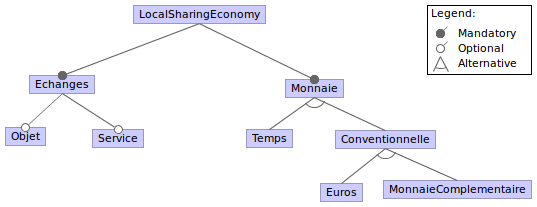
\includegraphics[scale=0.6]{exemple.png}}

Une petite précision est nécessaire pour pouvoir comprendre ce diagramme correctement.  On peut se poser la question des features alternatifs : s'agit-il d'alternatives exclusives ou non ?  Dans ce cas-ci,  nous dirons que oui.  Ainsi,  notre système ne pourra avoir qu'une seule monnaie parmi les choix : Temps,  Euros,  MonnaieComplémentaire.  Conceptuellement parlant,  nous pourrions imaginer un système avec plusieurs monnaies mais cela complexifie assez bien la tâche.

Pour la définition des features,  nous aurions ce qui suit : \\
\textbf{\underline{Local Sharing Economy : }} Economie locale d'échange,  il s'agit d'une communauté dont l'activité principale est l'échange entre personnes d'une zone géographique restreinte. \\
\textbf{\underline{Echanges : }} Action du passage d'un bien ou un service d'une personne à une autre,  en échange d'un montant de monnaie fixé.\\
\textbf{\underline{Monnaie}} Outil de mesure de la valeur d'un bien ou d'un service. \\
\textbf{\underline{Objet}} Un bien matériel dont on peut définir le propriétaire. \\
\textbf{\underline{Service}} Une action utile pour une personne. \\
\textbf{\underline{Temps}} Unités de temps exprimée en minutes, heures,  jours,  semaines et mois.  \\
\textbf{\underline{Monnaie conventionnelle}} Monnaie représentée sur forme matérielle et n'existant pas naturelement. \\
\textbf{\underline{Euro}} Monnaie officielle de la zone Euro. \\
\textbf{\underline{Monnaie complémentaire}} Monnaie conventionnelle mais non-officielle (non reconnue par les autorités civiles nationales). \\


Ensuite,  nous devons décrire les règles de composition.  Une règle que nous pouvons définir concernerait l'échange de biens et la monnaie utilisée.  En effet,  il semble difficile ou,  en tout cas,  peu logique,  de donner une valeur temporelle à un objet.  Nous pouvons donc décrire la règle que si le feature "Biens" est présent,  alors il faut une feature de type "Monnaie conventionnelle",  équivalent au feature "Biens" est mutuellement exclusif au feature "Temps".  D'une manière plus générale,  les règles de compositions sont souvent de 2 types : featureA \textbf{nécessite} featureB et featureA \textbf{est mutellement exclusif avec} featureB.  Tels que les noms l'indiquent,  la première règle signifie que si on désire intégrer featureA,  alors on doit également avoir featureB intégré.  La seconde règle signifie que l'on ne peut pas avoir featureA et featureB. 

%======== Paragraphe à relire car c'était celui d'en dessous avant.
%====================================================

Pour terminer notre feature model,  nous devons décrire les arguments qui doivent permettre de décider de la présence ou non de chaque feature.  D'abord,  nous voyons que "Echanges" et "Monnaies" sont obligatoires.  Nous n'avons pas le choix car toute économie d'échange local doit avoir défini ces 2 composantes.  Ensuite,  les features "Objet" et "Service" sont optionnels.  Le choix d'inclure un ou les 2 features sera simplement guidé par la réalité du terrain : voulons-nous que les échanges concernent des biens et/ou des services ?  De l'autre côté de notre diagramme,  nous avons la monnaie.  Notre règle compositionnelle nous signale déjà que notre choix sera guidé d'après la présence ou non du feature "Biens".  De plus,  si nous utilisons une monnaie conventionnelle,  le choix d'une monnaie alternative peut être motivé si on désire renforcer l'aspect local de l'économie.  \\

Ceci termine la description d'un exemple de feature model.  Nous avons utilisé un thème lié au mémoire mais,  bien sur,  il s'agit là d'une petite partie de l'analyse qui sera faite plus tard.  Ce chapitre nous a donc permis de mieux comprendre le principe des feature models et nous allons maintenant passer à la suite de la description des outils utilisés pour le mémoire. 

\subsection{Outil : featureIDE}

Pour pouvoir représenter le feature model que nous aurons élaboré,  il va falloir utiliser un outil efficace principalement pour représenter le feature diagram et pouvoir le modifier facilement. 

Au début de l'analyse,  nous avions utilisé une application disponible en ligne et permettant même de sauvegarder les projets sur la base de données du site.  Cet outil se nomme Software Product Line Online Tools \cite{splot}.  Malheureusement,  cet outil est fort simple et ne permet une visualisation que en arborescence textuelle.  Nous nous sommes donc orientés vers un autre outil plus adapté.  Il s'agit d'un module à installer dans l'environnement Eclipse \cite{eclipse} nommé featureIDE \cite{featureIDE}.  Une fois installé,  celui-ci permet de modifier notre feature diagram de plusieurs façon.  La première la plus intuitive est l'environnement graphique.  Ainsi,  les il est très simple d'ajouter / supprimer / modifier un des neouds du diagramme.  On peut aussi modifier directement des contraintes logiques à chaque branchement.  Dans certains cas,  il est intéressant de modifier directement le diagramme en mode "code source".   Ceci est faisable facilement simplement en ouvrant l'onglet "source code".  Le code sourceXML du diagramme apparaît alors et peut être modifié.   
Une fois que le diagramme est terminé,  on peut facilement exporter le résultat au format .PNG.  Les exemples illustrés dans la partie explicative sur les feature models donnent un aperçu du résultat des diagrammes dessinés via featureIDE.  Une autre utilité de ce programme est de pouvoir vérifier que le modèle est cohérent.  Il peut analyser le diagramme afin de voir s'il n'y a pas des éléments contradictoires.

\subsection{Outil : Django}

Lors du développement d'une solution pour BuurtPensioen dans le cadre du cours SINF/INFO 2255,  le groupe 8 (et d'autres) a choisi d'utiliser le framework Django.  Ce choix se comprend assez facilement pour plusieurs raisons.  D'abord,  Django est assez répandu et permet donc d'avoir accès à un grand nombre de ressources d'aide au développement (tutoriels,  FAQs,  forums, \dots ).  Ensuite,  Django permet d'utiliser des extensions très facilement.  Ceci est utile pour rajouter des fonctionnalités sans devoir réinventer la roue.  Nous allons donc aborder maintenant cet outil plus technique et qui sera utilisé pour l'étape de développement de notre framework.  Étant donné l'ampleur de l'outil et l'importance de celui-ci dans le projet,  il est intéressant de passer un peu de temps à se familiariser avec le framework Django.  

\label{django}
Django \cite{django} est un framework écrit en python \cite{python} et destiné à faciliter la mise en place de sites internet.  

D'un point de vue architectural,  un \textbf{projet} django utilise une ou plusieurs \textbf{application(s)}.  Ensuite,  chaque application fonctionne sous le principe Model-View-Controller.  C'est-à-dire qu'on divise l'application en 3 \textit{couches} : le modèle contient les données (classes,  bases de données, ....),  la vue s'occupe de la partie visible par l'utilisateur et enfin la partie controlleur gère la logique de l'application.  Dans le cas d'une application Django,  on décrit les données (=le modèle) dans un seul fichier : models.py.  Celui-ci est utilisé pour générer automatiquement la base de données.  La vue est gérée dans différents fichiers que l'on nomme  \textbf{templates}.  On aura un fichier par page web et Django rajoutera,  aux endroits définis par le code,  les informations issues de la base de données.  En plus des \textbf{templates},  il faut définir les URL qui seront utilisées et préciser quelle fonction va gérer chacune d'elle.  Ceci se fait dans le fichier urls.py.  Enfin,  on décrit le fonctionnement de l'application (couche controlleur) dans un fichier qui porte le nom,  à tort,  views.py.  Ce nom lui a été attribué car il contient,  en fait,  la logique pour chacune des pages de la vue.  Il y a donc un lien fort avec la vue mais c'est bel et bien là que se retrouvera toute la logique du site web.  Dans ce fichier,  on retrouve chacune des fonctions pointées par les URL définies précédemment.  Les fonctions peuvent faire appel ou mettre à jour la base de données,  manipuler les données,  puis les envoyers à un template qui permettra d'afficher le tout à l'utilisateur.  

Afin de voir plus en détails le fonctionnement de Django,  nous allons créer une simple application web.  Étant donné que le sujet de ce mémoire concerne des offres et demandes de biens ou services,  nous allons créer un mini-site qui aura pour but d'enregistrer des offres ou demandes ainsi que de voir la liste des éléments enregistrés.

Après avoir installé Django sur notre machine,  nous pouvons créer notre premier projet.  Une commande crée automatiquement une structure de base.  Nous créons ensuite aussi automatiquement les fichiers et dossiers de notre application.  Il ne reste plus qu'à programmer dans celle-ci.  

D'abord,  concernant la couche "modèle" (données) de notre application,  nous avons simplement des "BusinessUnits" et des "Actors".  Les BusinessUnits représentent les entités vendues ou échangées tandis que les Actors représentent les vendeurs ou acheteurs de notre système.  Chaque BusinessUnit possède les caractéristiques suivantes : un nom,  un vendeur (=Actor),  un acheteur (=Actor) et une date de validation.  Les Actors eux ont simplement un nom.  Nous allons donc décrire ceci dans le fichier models.py : 

\lstset{language=Python,frame=single,keywordstyle=\color{blue},commentstyle=\color{green},breaklines=true}

\begin{lstlisting}
class Actor(models.Model):
	name = models.CharField(max_length=50)

class BusinessUnit(models.Model):
	descr_text = models.CharField(max_length=200)
	vendor_name = models.ForeignKey('Actor',related_name='actor_vendor')
	buyer_name = models.ForeignKey('Actor',related_name='actor_buyer')
	date_validated = models.DateTimeField('validation date')
\end{lstlisting}

Ce code est suffisant et sera utilisé par Django pour générer puis gérer les accès à la base de données.  Une simple commande permet d'appliquer ce schéma à la base de données et directement après,  nous pouvons insérer ou lire les données selon le schéma que nous venons de définir.

Maintenant que le modèle des données est défini,  nous allons passer aux vues (templates) et aux controlleurs (views.py).  Pour essayer d'être le plus clair possible sur le fonctionnement,  nous allons retracer les appels de fonctions au sein du code source.  Ainsi,  étant donné que nous réalisons une application web,  nous allons démarer d'une URL.  Nous allons définir dans l'application Django une URL qui permettra d'accéder à une page reprenant toutes les BusinessUnit présentes dans la base de données.

Pour cela,  nous modifions d'abord le fichier urls.py et définissons comme suit : 

\begin{lstlisting}
from django.conf.urls import url
from . import views

urlpatterns = [
    url(r'^$', views.index, name='index'),
]
\end{lstlisting}

Cette définition permet d'indiquer à Django la fonction utilisée pour gérer l'URL pointant sur l'index de notre application.  La fonction utilisée sera celle donc views.index,  c'est-à-dire la fonction index dans le fichier views.  

Nous devons maintenant définir cette fonction dans le fichier views.py.  Dans cette fonction,  nous devrons récupérer tous les BusinessUnits,  puis choisir un template qui affichera les données,  ensuite créer le contexte,  c'est-à-dire la correspondance entre les données récupérées dans la base de données avec le nom des variables présentes dans le template.  Enfin,  il faut renvoyer à l'utilisateur le mélange des 2 : notre template avec du contenu dans les variables.  Nous verrons juste après le template proprement dit.  D'abord le code de la logique décrite ci-avant : 

\begin{lstlisting}
from django.template import RequestContext, loader
from django.shortcuts import render
from django.http import HttpResponse

from .models import BusinessUnit, Actor

def index(request):

    # On recupere 5 BusinessUnits de la base de donnees
    liste = BusinessUnit.objects.order_by('date_validated')[:5]
   # On cree un contexte avec les donnees recuperees
    context = RequestContext(request, {
        'liste': liste,
    })

   # On charge un template qui sera utilise pour presenter les donnees
    template = loader.get_template('basiceconomy/index.html')

   # On retourne a l'utilisateur le template avec son contexte
    return HttpResponse(template.render(context))

\end{lstlisting}

Il ne nous reste plus qu'à créer notre template dans le dossier "templates" de l'appliaction et à l'endroit que nous avons indiqué,  c'est-à-dire dans le sous dossier basiceconomy/.  Un fichier de template est un mix entre du HTML et du python.  Le HTML représente de la mise en forme finale tandis que le python est utilisé pour insérer des données ou messages divers à partir des variables définies dans le contexte de la page.  A la base,  le code est considéré comme du HTML et lorsqu'on décide d'insérer du python,  on place le code entre \{\% et \%\} ou bien \{\{ et \}\} pour insérer purement le contenu d'une variable.  Le code du template de notre page d'index repenant la liste des BusinessUnits se présente donc comme suit : 

\begin{lstlisting}


    <ul>
    
        <li>{{ bu.descr_text }}</li>
    
    </ul>

    <p>No business units are available.</p>


\end{lstlisting}

Tout ceci étant fait,  il ne reste plus qu'à lier notre application à notre projet afin qu'elle soit accessible.  Pour cela,  il suffit de modifier 2 fichiers dans le dossier du projet : le fichier de configuration (settings.py) dans lequel on indique qu'on utilise notre application,  et le fichier urls.py dans lequel nous indiquons qu'il faut inclure les urls de notre application dans celles du projet en général.  
En guise de résumé de ce petit tutoriel,  nous allons jeter un oeil à l'arborescence finale de notre projet.  A noter que nous avons nommé notre projet "testproject" et notre application se nomme "basiceconomy".  L'arborescence,   au départ du dossier principal du projet,  est la suivante.
\\
\\
\underline{\textbf{.:}} \newline
\textbf{testproject} \newline
\textbf{basiceconomy} \newline
db.sqlite3 \newline
manage.py \newline

A la racine,  nous retrouvons 1 dossier du même nom que notre projet principal ainsi qu'un dossier du même nom que notre application.  Pour chaque application développée pour le projet,  nous créerons un nouveau dossier ici qui portera son nom.  On retrouve aussi le fichier manage.py qui permet d'administrer le serveur django (effectuer les migrations de la base de données,  créer un superuser,  lancer le serveur, \dots )
\\
\\
\underline{\textbf{./testproject:}} \\
\textbf{\_\_pycache\_\_} \\
\_\_init\_\_.py \\
settings.py \\
urls.py \\
wsgi.py \\

Le dossier du même nom que notre projet reprend le code qui le concerne.  Nous n'y avons modifié que 2 fichiers : settings.py dans lequel nous avons renseigné que nous utilisions l'application basiceconomy et urls.py dans lequel nous avons indiqué qu'il fallait inclure les urls de l'application basiceconomy dans les urls du projet général.Le reste des fichiers et dossiers a été généré automatiquement lors de la création du projet.
\\
\\
\underline{\textbf{./basiceconomy:}} \\
\textbf{migrations} \\
\textbf{templates} \\
\textbf{\_\_pycache\_\_} \\
admin.py \\
\_\_init\_\_.py \\
models.py \\
tests.py \\
urls.py \\
views.py \\

Nous sommes maintenant dans le dossier principal de notre application basiceconomy.  Nous avosn commencé par modifier models.py afin d'y décrire notre modèle de données.  Il fallait alors effectuer une migration (au moyen du fichier manage.py présent à la racine du projet) de la base de données.  Ensuite,  nous avons modifié urls.py pour pouvoir lier une url avec une fonction.  La fonction en question est décrite dans views.py et récupèrera un template.  Ce template se retrouve plus loin dans l'arborescence (dans le dossier templates).
\\
\\
\underline{\textbf{./basiceconomy/migrations:}} \\
\textbf{\_\_pycache\_\_} \\
0001\_initial.py \\
0002\_auto\_20150409\_1142.py \\
0003\_auto\_20150409\_1445.py \\
\_\_init\_\_.py \\

Ce dossier est utilisé pour retenir les différentes migrations,  c'est-à-dire les différences entre le modèle décrit dans models.py et la base de données.  Tout ceci est géré automatiquement via une simple commande.
\\
\\
\underline{\textbf{./basiceconomy/templates:}} \\
\textbf{basiceconomy} \\

Les templates sont regroupés dans des sous-dossiers pour des raisons d'organisation.
\\
\\
\underline{\textbf{./basiceconomy/templates/basiceconomy:}} \\
details.html \\
index.html \\

On retrouve finalement nos templates qui,  une fois couplés avec un contexte de données,    permettront d'afficher une page à l'utilisateur.

Ce petit exemple terminé,  nous avons pu avoir un aperçu du fonctionnement global de Django.  

\subsection{Open-source et licences}

Dès le début de l'analyse des besoins,  il est apparu qu'il fallait éviter que l'histoire se répète pour l'outil qui allait être développé. En effet,  d'autres outils existent et certains ont été,  à une époque,  en accès gratuit pour les organisations qui le désiraient.  Mais vu le succès rencontré,  les propriétaires ont repéré l'opportunité de faire du profit et certains outils sont maintenant devenus (parfois partiellement) payants.  La question de la licence d'utilisation a donc été une des premières questions à poser.  

Pour cela,  une rencontre avec le Louvain Technology Transfert Office a été organisée et de bons éléments de réponses ont pu être apportés.   L'idée étant d'analyser ce que l'on désire pour l'avenir de notre application et de choisir une licence appropriée en fonction de ces perspectives pour le futur.

D'abord,  2 catégories de licences existent : les licences propriétaires et les licences open-sources.  Dans les 2 cas,  il faut prêter attention au transfert de licence.  C'est-à-dire du fait qu'utiliser un programme ou un bout de programme dans son propre projet,  peut avoir des conséquences sur la licence de notre projet.  Par exemple,  il se peut que la licence de la bibliothèque utilisée soit transférée à tout notre projet,  si on l'utilise.  De plus,  les questions de la disponibilité du code source ainsi que la possibilité de l'utiliser/modifer gratuitement occupent une place centrale dans la réflexion.  Dans notre cas,  comme dis ci-dessus,  l'inquiétude principale était d'empêcher qu'une personne puisse s'approprier le projet et le rende payant pour les utilisateurs.  Dès lors,  les licences open-source semblent correspondre et parmis elles,  on peut citer la plus connue : GPL (GNU Public Licence).  Cette licence est celle utilisée "par défaut" pour les projets open-source.  Elle semble correspondre car elle ne supporte pas le mélange avec des logiciels propriétaire et oblige à rendre le code de l'application disponible lorsqu'on la distribue.  Elle peut donc empêcher qu'une partie ou  l'entièreté du projet soit privatisée.  Cependant,  nous ne sommes pas au bout de la réflexion.  En effet,  sachant que notre projet prendra très probablement la forme d'un site web,  il est intéressant de voir si une licence n'est pas plus adaptée à cette sitaution.  Pour cela,  le cas de l'AGPLv3 (Affero GNU Public Licence) semble correspondre à nos besoins.  Il s'agit d'une licence basée sur GPL  mais exigeant que,  pour les applications online,  l'accès au code source doit être explicitement référencé quelque part.  Ce système permet d'éviter le cas,  par exemple,  de certains applications Google.  En effet,   l'utilisation de ces systèmes est gratuite mais il n'est techniquement pas possible de récupérer le code source.  Sous licence AGPL,  l'application doit inclure quelque part un lien vers le code source du projet.  

En définitive,  c'est la licence AGPLv3 qui sera choisie pour couvrir le projet de framework.  Ceci permettra aussi peut-être de pouvoir créer une communauté de développement autour du framework afin d'améliorer celui-ci,  à l'instar de Linux et d'autres projets open-source portés par une forte communauté.

Cette section sur les licences clôture ce chapitre à propos des outils utilisés dans le cadre de ce mémoire.  Nous avons également déjà pu,   via les exemples, aborder la thématique des échanges locaux.  Il s'agit du sujet principal du chapitre suivant qui vise à décrire le problème traité dans ce travail.